\section{Case Study: mVAM in Yemen}

\section{Motivation: Survey Data on Household Food Security}

   

\subsection{Household Food Security in Yemen}

The dataset considered comprises surveys collected in Yemen during the COVID-19 pandemic period between March 2020 and December 2022, during which time 145,013 responses were recorded. An average of roughly 143 households per day were randomly selected using stratified geographic sampling, with varying numbers of responses recorded at the governorate level. Demographic information for each household included geographic location at the district level, the gender of the head of household, the size of the household, and the primary and secondary income sources. Each respondent was also asked to report whether the household was internally displaced or hosting IDPs. Questions about the household's ability to access medical care and educational services were also included due to COVID-19 restrictions. Questions about food consumption and coping strategies needed to construct two standard WFP food security indicators were included as described in Section~\ref{FS_defs}, and respondents were also asked to report whether they had received food assistance from WFP, the duration of time since their last distribution, and the type of assistance they had received (cash, vouchers, or food items).    

\subsection{Food Security Indicators}\label{FS_defs}
The Food Consumption Score (FCS), initially developed by WFP in 1996, is a summary statistic intended to measure dietary adequacy from both a nutritional and caloric standpoint~\citep{WFP_FCS_2024}. Respondents are asked to state the number of days in the previous week that members of their household consumed foods from a standard list of groups, based on the assumption that meals in the household are communal. The FCS is computed by taking a weighted average of the days of consumption of eight major food groups (Starches, Vegetables, Fruits, Pulses, Dairy, Animal Proteins, Fats, and Sugar), according to the following formula: $\mbox{FCS} = (\mbox{Starches}\times 2)+ (\mbox{Pulses}\times 3)+ \mbox{Vegetables} + \mbox{Fruit} + (\mbox{Meat}\times 4)+ (\mbox{Dairy}\times 4)+ (\mbox{Fats}\times .5)+ (\mbox{Sugar} \times.5).$ The weights sum to 16, and the maximum attainable score is 112. In its reporting, WFP defines FCS thresholds to classify households into three consumption levels. In Yemen, households scoring at or below 28 are considered to have a poor level of consumption, as a score this low would be associated with consuming little other than starches, fats, and sugar on a daily basis. Households scoring between 29 and 42 have inadequate or borderline levels of consumption, while households scoring 43 or above are considered to have adequate consumption~\citep{WFP_FCS_2024}.

The Reduced Coping Strategies Index (rCSI) is a food security indicator developed by the WFP and CARE to measure the frequency and severity of food-related coping strategies used by households when faced with insufficient food or resources to purchase food~\citep{rCSI}. It is based on a seven-day recall period covering five standard behaviors: (1) relying on less preferred or less expensive foods; (2) borrowing food or relying on help from friends or relatives; (3) limiting portion sizes at mealtimes; (4) restricting consumption by adults so that children can eat; and (5) reducing the number of meals eaten per day. Each behaviour is assigned a severity weight (1, 2, 1, 3, and 1, respectively), and the household’s rCSI is calculated by multiplying the reported frequency (days) of each behaviour by its weight and summing across all five strategies. Higher scores indicate greater reliance on coping strategies and, therefore, poorer food security. Although there are no universally implemented thresholds for rCSI scores, the Integrated Food Security Phase Classification (IPC) considers a score of 19 or above to represent moderate food insecurity {\citep{cfi}}.

\subsection{Covariates}
If we were to coerce the data to allow a time series with covariates to be fit, we would need to calculate daily aggregates for all the varying effects, including the random ones. In the case of \emph{adm1}, a categorical variable with 22 levels, the preservation of information would necessitate the creation of 21 variables, each displaying the proportion of a daily sample represented by a given region (with the final proportion simply being the difference between 1 and the sum of all others). 

\begin{figure}[htbp]
    \centering
    \label{fig:adm1_prop_hist}
    \begin{subfigure}{\textwidth}
        \centering
        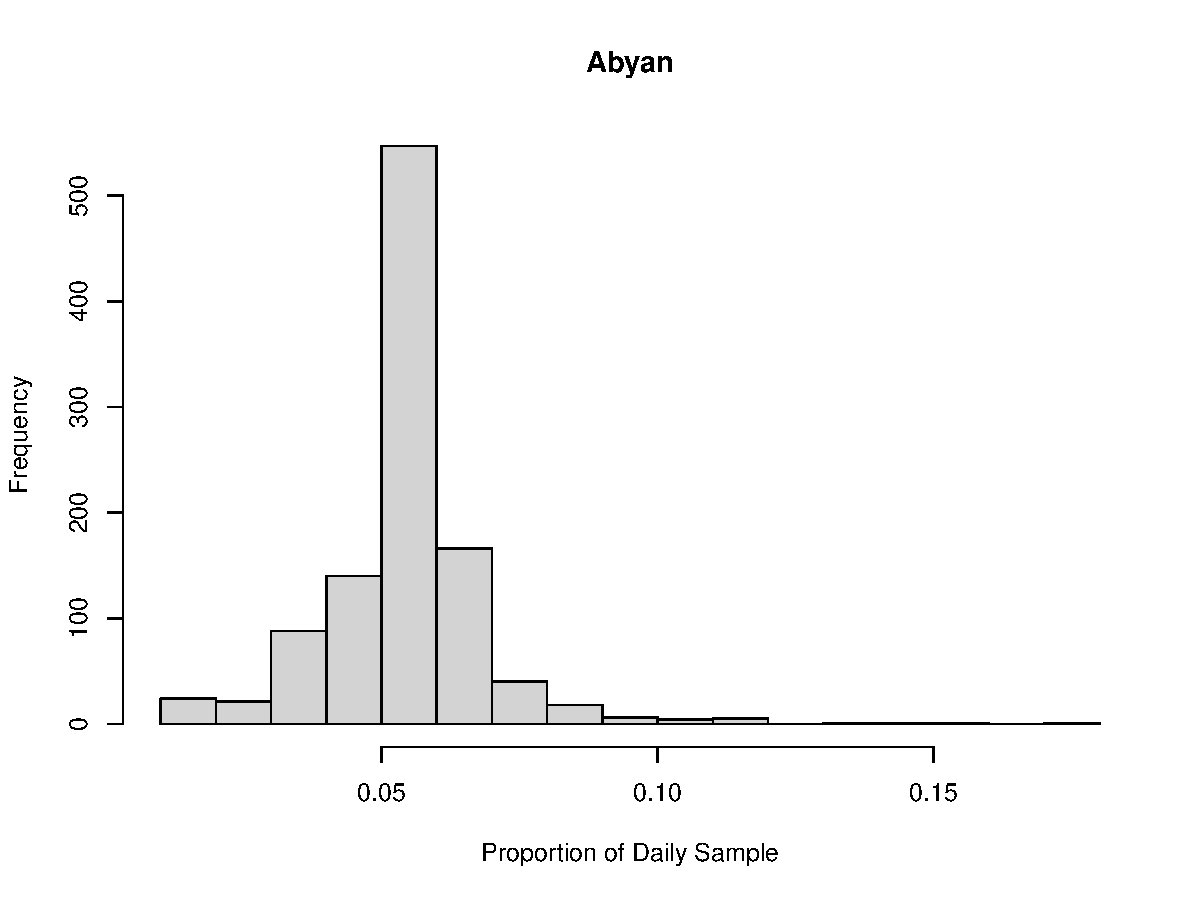
\includegraphics[width=\linewidth, page=1]{images/output/adm1_prop_hists.pdf}
    \end{subfigure}
    \caption{A histogram of the proportions of each daily sample made up by households located in the Abyan governorate.}
\end{figure}

If we look at Figure \ref{adm1_prop_hist} we see a histogram of daily frequencies for the governorate Abyan that is emblematic of many other regions, in which we see an empirical distribution with little variance. Were there to be a significant difference between household food security levels in Abyan and those of the national average, the lack of variance in frequency would preclude a time series model with covariates from picking up the effect. There is also the matter of how many degrees of freedom that would be introduced by generating frequency variables for each of the 22 governorates and 331 districts, variables that may very well provide insight into the food security dynamics of the country.